\documentclass{article}
\begin{document}
\section{Debugging via VS code}
Here are the steps to follow to debug programs via VS code:
\begin{itemize}
	\item Download Segger software from from \url{https://www.segger.com/downloads/jlink/}.
	\item Refer to \url{https://wiki.segger.com/J-Link_Visual_Studio_Code} for using J-link with VS code.
	\item Download the NRF5 .svd file from Nordic Semiconductor github.
	\item Connect J-link to SWD debugger connector.
	\begin{figure}[H]
		\begin{center}
			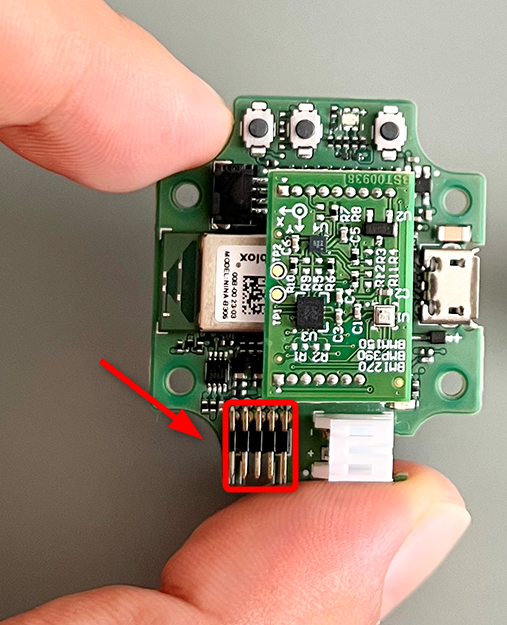
\includegraphics[width=0.25\textwidth]{coinesAPI_images/App31_jlink_connection.png}
			\caption{APP3.1 Debugger connector}
		\end{center}
	\end{figure}
	\item Below is the sample launch.json config for VS code debug.
	\begin{figure}[H]
		\begin{center}
			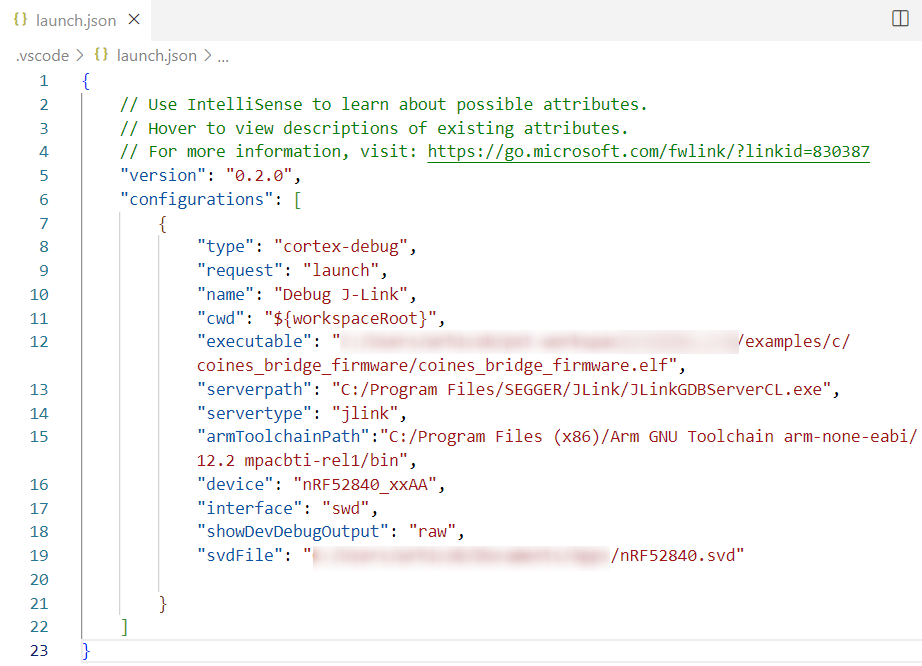
\includegraphics[width=0.8\textwidth]{coinesAPI_images/Debug_launch_json.png}
			\caption{VS code debug launch.json}
		\end{center}
	\end{figure}
\end{itemize}

\newpage

\end{document}